\chapter[Metodologia]{Metodologia}\label{ch:metodologia}

Este capítulo tem o objetivo de apresentar a metodologia bem como os fluxos que foram seguidos a fim de atingir os objetivos da pesquisa. A Seção \ref{sec:metodologias} discute sobre metodologias de pesquisa científica para, em seguida, na Seção \ref{sec:escolhas_metodologicas}, serem apresentadas as escolhas metodológicas adotadas por este trabalho. As seções \ref{sec:proc_tcc}, \ref{sec:proc_rs} e \ref{sec:metodologia_desenvolvimento} detalham os fluxos de condução do TCC como um todo, Revisão Sistemática e desenvolvimento, respectivamente.

\section{Metodologias de pesquisa}\label{sec:metodologias}

O conhecimento científico diverge dos demais tipos de conhecimento devido à necessidade de adotar fundamentação e metodologias a serem seguidas. Além disso, baseia-se em \textit{“informações classificadas, submetidas à verificação, que oferecem explicações plausíveis a respeito do objeto ou evento em questão”} \cite[pág. 22]{prodanov2013}. Ou seja, é imprescindível determinar o método científico que possibilitou atingir esse conhecimento \cite[pág. 24]{prodanov2013}. 

O desenvolvimento do método científico, mediante sua aplicação formal e sistemática, possibilita a pesquisa científica \cite{gil2008}. O objetivo fundamental da pesquisa é descobrir respostas para problemas mediante o emprego de procedimentos científicos \cite[pág. 26]{gil2008}.

Quanto aos objetivos, é possível classificar as pesquisas em três categorias \cite[pág. 41]{gil2002}: (i) exploratória, (ii) descritiva e (iii) explicativa. A Tabela \ref{tab:classificacao_pesquisa} apresenta os objetivos das mesmas.



%\begin{citacao}``A utilização desse tipo de abordagem difere da abordagem quantitativa pelo fato de não utilizar dados estatísticos como o centro do processo de análise de um problema, não tendo, portanto, a prioridade de numerar ou medir unidades." \cite{prodanov2013}.\end{citacao}%

% ######## init table ########
\begin{table}[h!]
 \centering
 \caption{Classificação da pesquisa científica quanto aos objetivos.}
 \label{tab:classificacao_pesquisa}
% distancia entre a linha e o texto
 {\renewcommand\arraystretch{0.25}
 \begin{tabular}{ l l l l }
  \hline
    \multicolumn{1}{p{1.883cm}}{\begin{center} 
\end{center}} &
    \multicolumn{1}{p{3.517cm}}{\begin{center}\textbf{Pesquisa Exploratória}
\end{center}} &
    \multicolumn{1}{p{3.600cm}}{\begin{center}\textbf{Pesquisa Descritiva}
\end{center}} &
    \multicolumn{1}{p{3.583cm}}{\begin{center}\textbf{Pesquisa Explicativa}
\end{center}}
  \\  
  \cline{1-1}\cline{2-2}\cline{3-3}\cline{4-4}  
    \multicolumn{1}{p{1.883cm}}{\begin{center}\textbf{Objetivo}
\end{center}} &
    \multicolumn{1}{p{3.517cm}}{\begin{center}Propiciar maior familiaridade com o problema, com o propósito de torná-lo mais explícito ou a construir hipóteses \cite[pág. 41]{gil2002}.
\end{center}} &
    \multicolumn{1}{p{3.600cm}}{\begin{center}Registrar e descrever os fatos observados sem interferência do pesquisador \cite[pág. 52]{prodanov2013}.
\end{center}} &
    \multicolumn{1}{p{3.583cm}}{\begin{center}\textit{``Identificar os fatores que determinam ou que contribuem para a ocorrência dos fenômenos”} \cite[pág. 42]{gil2002}.
\end{center}}
  \\  
  \hline

 \end{tabular} }
\end{table}

Com relação à abordagem, a pesquisa pode ser classificada em: (i) pesquisa quantitativa e (ii) pesquisa qualitativa. A pesquisa quantitativa considera que tudo pode ser quantificável; opiniões e informações podem ser traduzidas em números para que sejam classificadas e analisadas. Este tipo de pesquisa exige o uso de recursos e de técnicas estatísticas \cite{prodanov2013}. A pesquisa qualitativa investiga a relação dinâmica entre o mundo real e o sujeito, isto é, um vínculo inerente entre o mundo objetivo e a subjetividade do objeto de estudo que não pode ser traduzido em números. 

Segundo \citeonline{prodanov2013}, do ponto de vista da natureza, a pesquisa pode ser classificada como: (i) básica e (ii) aplicada. Pesquisa básica tem por objetivo resultar em novos conhecimentos que sejam úteis para a ciência, porém sem a definição prévia de uma aplicação prática. A pesquisa aplicada busca resultar em conhecimentos com aplicação em soluções para problemas específicos. 

Cabe ressaltar, que para obter os dados para a elaboração da pesquisa são adotados os procedimentos técnicos. Existem dois grandes grupos de procedimentos técnicos, segundo \citeonline[pág. 54]{prodanov2013}:
(i) aqueles que se utilizam das chamadas fontes de papel (pesquisa documental e pesquisa bibliográfica) e (ii) aqueles cujos dados são produzidos por pessoas (pesquisa participante, pesquisa \textit{ex-post-facto}, o levantamento, pesquisa experimental, o estudo de caso e a pesquisa-ação).

A pesquisa-ação busca conectar a pesquisa à ação ou prática, o que significa que o conhecimento e sua compreensão são desenvolvidos como parte da prática \cite{engel2000pesquisa}. Neste contexto, o pesquisador torna-se participante da pesquisa, onde pode intervir com o fim de verificar se um novo procedimento é eficaz. 

A pesquisa-ação é um tipo de pesquisa auto-avaliativa onde procura-se intervir na prática ainda no decorrer do próprio processo de pesquisa e não somente em sua etapa final \cite{engel2000pesquisa}. Além disso, a pesquisa-ação é cíclica: para que os resultados de fases anteriores da pesquisa sejam aprimorados, os resultados das fases anteriores são avaliados \cite{engel2000pesquisa}.



%Definição de um problema, pesquisa preliminar, hipótese, desenvolvimento de um plano de ação, implementação do plano de ação, coleta de dados para avaliação dos efeitos da implementação do plano, avaliação do plano de intervenção, comunicação dos resultados

\section{Escolhas metodológicas}\label{sec:escolhas_metodologicas}

%Quanto à natureza classifica-se como aplicada pois pretende gerar conhecimentos para aplicação prática, dirigidos à solução de problemas específicos \cite[pág. 35]{silveira}. 

A Tabela \ref{tab:metodologia_pesquisa} apresenta, brevemente, as escolhas metodológicas definidas para este trabalho. O tipo de pesquisa adotado neste trabalho, quanto aos objetivos da pesquisa, é o exploratório. Em termos de abordagem, a pesquisa qualitativa foi a mais adequada a este trabalho. Quanto à natureza, a pesquisa classifica-se como aplicada, pois buscou gerar conhecimentos a serem utilizados na solução de problemas específicos. Quanto aos procedimentos, inicialmente, optou-se por pesquisa bibliográfica para permitir que o pesquisador conheça os estudos já realizados sobre o assunto \cite[pág. 31]{fonseca}. 



% ######## init table ########
\begin{table}[h]
 \centering
 \caption{Metodologia de pesquisa}
 \label{tab:metodologia_pesquisa}
% distancia entre a linha e o texto
 {\renewcommand\arraystretch{0.25}
 \begin{tabular}{ l l l l }
  \hline
    \multicolumn{1}{p{2.517cm}}{\begin{center}\textbf{Quanto aos objetivos}
\end{center}} &
    \multicolumn{1}{p{2.600cm}}{\begin{center}\textbf{Quanto à abordagem}
\end{center}} &
    \multicolumn{1}{p{2.583cm}}{\begin{center}\textbf{Quanto à natureza}
\end{center}} &
    \multicolumn{1}{p{3.583cm}}{\begin{center}\textbf{Procedimentos}
\end{center}}
  \\  
  \cline{1-1}\cline{2-2}\cline{3-3}\cline{4-4}  
    \multicolumn{1}{p{2.517cm}}{\begin{center}Pesquisa exploratória \end{center}} &
    \multicolumn{1}{p{2.517cm}}{\begin{center}Pesquisa qualitativa\end{center}} &
    \multicolumn{1}{p{2.600cm}}{\begin{center}Pesquisa aplicada\end{center}} &
    \multicolumn{1}{p{4.583cm}}{\begin{center}Pesquisa bibliográfica, Revisão Sistemática, Pesquisa-ação, \textit{Scrum}\end{center}}
  \\  
  \hline

 \end{tabular} }
\end{table}

Foi utilizada Revisão Sistemática da literatura de modo a identificar possíveis arquiteturas para SMA. Para apoiar o desenvolvimento, foi feita uma adaptação da metodologia \textit{Scrum}. Quanto à análise dos resultados da pesquisa foi adotado o procedimento de pesquisa-ação. Diante do exposto, para plena condução desse trabalho, foram desenhados quatro fluxos principais: (i) fluxo de atividades para a condução do TCC\_1; (ii) fluxo de atividades para a condução do TCC\_2; (Seção \ref{sec:proc_tcc}); (iii) fluxo de atividades de Revisão Sistemática (Seção \ref{sec:proc_rs}), e (iv) fluxo  para condução das atividades associadas ao desenvolvimento e/ou à implementação dos padrões arquiteturais (Seção \ref{sec:proc_ds}). Cabe ressaltar que o fluxo de atividades para condução do TCC compreende os demais fluxos, conforme detalhado na próxima Seção.


%%%%%%%%%%%%%%%%%%%%%%%%%%%%%%%%%%%%%%%%%%%%%%%%%%%%%%%%%


\section{Fluxo de atividades para condução do TCC}\label{sec:proc_tcc}

A condução do TCC foi modelada em duas etapas: a etapa referente ao TCC\_1 (Figura \ref{fig:proc_tcc1}) e a etapa referente ao TCC\_2 (Figura \ref{fig:proc_tcc2}).

\begin{figure}[!htb]
\centering
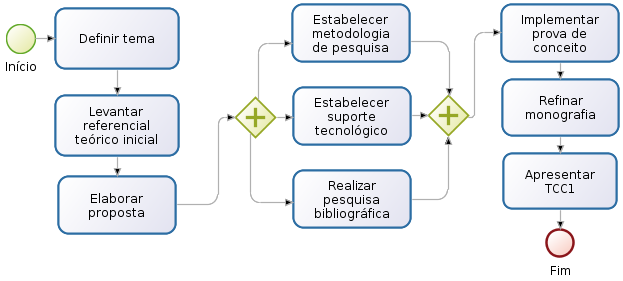
\includegraphics[scale=0.6]{figuras/processo_tcc1}
\caption{Fluxo de atividades para o desenvolvimento do TCC\_1.}
\label{fig:proc_tcc1}
\end{figure}



As atividades descritas no fluxo para condução do TCC\_1 (Figura \ref{fig:proc_tcc1}) são apresentadas, resumidamente, a seguir:

\begin{itemize}
    \item \textbf{Definir tema:} envolve a identificação da área de pesquisa, discussão sobre possíveis temas de relevância;
    \item \textbf{Levantar referencial teórico inicial:} o referencial teórico que fundamenta a proposta e consolida o tema é levantado nesta atividade;
    \item \textbf{Elaborar proposta:} fomentar a pesquisa de modo a estabelecer seu escopo, objetivos, justificativa, questões de pesquisa, metodologia e cronograma de atividades mais elementares. Tais aspectos podem sofrer modificações ao decorrer do trabalho;
    \item \textbf{Estabelecer metodologia de pesquisa:} com maior familiaridade do pesquisador sobre o tema, a metodologia de pesquisa pode ser consolidada e classificada;
    \item \textbf{Estabelecer suporte tecnológico:} trata-se da indicação das ferramentas a serem utilizadas, as quais apoiam o desenvolvimento da proposta;
    \item \textbf{Realizar pesquisa bibliográfica:} envolve a pesquisa de trabalhos científicos que forneçam embasamento para os objetivos pré-estabelecidos. O fluxo de atividades para Revisão Sistemática (Seção \ref{sec:proc_rs}) foi adotado para esta atividade;
    \item \textbf{Implementar prova de conceito:} implementação de prova de conceito para que sejam  identificados riscos potenciais que possam interferir na catalogação dos padrões. O fluxo, centrado em atividades de desenvolvimento e/ou implementação, adotado nesse trabalho, encontra-se descrito na (Seção \ref{sec:proc_ds});
    \item \textbf{Refinar monografia:} com base nos resultados obtidos até o momento, foi averiguado bem como documentado se os objetivos estabelecidos para cumprimento no TCC\_1 foram atingidos. Isso permitiu refinar a parte escrita da monografia, e
    \item \textbf{Apresentar TCC\_1}: consiste na apresentação do TCC\_1 à banca examinadora.
\end{itemize}


As atividades descritas no fluxo para condução do  TCC\_2 (Figura \ref{fig:proc_tcc2}) são apresentadas, brevemente, a seguir.

\begin{figure}[!htb]
\centering
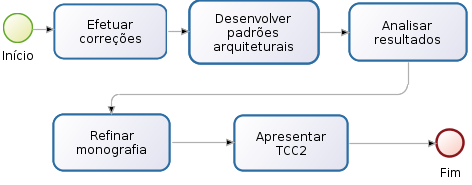
\includegraphics[scale=0.6]{figuras/processo_tcc2}
\caption{Fluxo de atividades para o desenvolvimento do TCC\_2.}
\label{fig:proc_tcc2}
\end{figure}





\begin{itemize}
    \item \textbf{Efetuar correções:} adequação da monografia às sugestões e críticas da banca examinadora;
    \item \textbf{Desenvolver padrões arquiteturais:} uma vez que os padrões arquiteturais já foram identificados, essa atividade compreende a modelagem, a implementação bem como a catalogação desses padrões. Vale ressaltar que a prova de conceito realizada, permitiu configurar o ambiente de desenvolvimento bem como acordar possíveis riscos e estabelecer caminhos seguros para a condução dessa atividade;
    \item \textbf{Analisar resultados:} foi adotado o procedimento de pesquisa-ação para avaliação de cada padrão arquitetural catalogado. Portanto, os passos relacionados à análise de resultados foram detalhados após o desenvolvimento dos padrões, de forma cíclica, atendendo, portanto, à característica inerente da pesquisa-ação; onde o pesquisador pode intervir na prática ainda no decorrer do próprio processo de pesquisa, baseando-se nos resultados obtidos até determinado momento. Os dados coletados, podem ser de natureza qualitativa ou quantitativa. Além disso, a avaliação dos padrões pode ocorrer unicamente por parte do pesquisador, ou por parte de desenvolvedores de SMA. 
    \item \textbf{Refinar monografia:} com base nos resultados obtidos ao final do projeto, foi averiguado bem como documentado se os objetivos estabelecidos para cumprimento no TCC como um todo foram atingidos. Isso permitiu refinar a parte escrita da monografia;
    \item \textbf{Apresentar TCC\_2:} apresentação do TCC\_2 à banca examinadora, e
    \item \textbf{Efetuar correções finais:} possui como intuito realizar as correções e os refinamentos apontados pela banca após a apresentação do TCC\_2.

\end{itemize}

\section{Revisão Sistemática}\label{sec:proc_rs}

A maioria das pesquisas começa com uma revisão da literatura. No entanto, a revisão de literatura possui pouco valor científico \cite{kitchenham2004}. Uma Revisão Sistemática (RS) pode ser adotada neste caso. Uma RS, é um meio de identificar, avaliar e interpretar boa parte das pesquisas disponíveis e, ao mesmo tempo, relevantes para um determinado foco \cite{kitchenham2004}. 

A RS sintetiza trabalhos existentes de acordo com uma estratégia de busca pré-definida. A estratégia de busca deve permitir que a integridade da pesquisa seja avaliada. Dentre as razões para realizar uma Revisão Sistemática da literatura, \citeonline{kitchenham2004} destaca:

\begin{itemize}
    \item Resumir a evidência existente sobre algum tópico em particular;
    \item Identificar eventuais lacunas na pesquisa atual, a fim de sugerir novas áreas de investigação, e
    \item Fornecer um \textit{framework} ou \textit{background} para outras pesquisas.
\end{itemize}


%Estudos individuais que contribuem com uma Revisão Sistemática são chamados estudos primários; uma Revisão Sistemática é uma forma de estudo secundário \cite{kitchenham2004}.

A condução do processo de Revisão Sistemática pode ser entendida como uma abordagem em três fases, como apresentado na Figura \ref{fig:fases_rs}. A primeira fase da pesquisa começa a partir de conceitos, que, de forma explícita e formalmente, representam o assunto em questão. São definidos os procedimentos que o pesquisador deve utilizar. Em seguida, é realizada a análise dos estudos que podem conter as informações e evidências sobre o tema específico da investigação \cite{biolchini2005}. 


\begin{figure}[!htb]
    \centering
    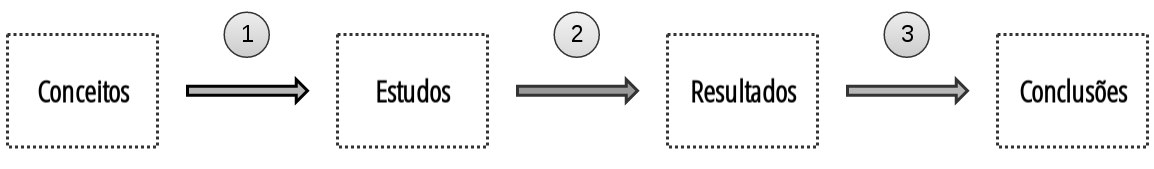
\includegraphics[scale=0.4]{figuras/fases_rs.png}  
    \caption{Abordagem de Revisão Sistemática em três fases. Traduzido. Fonte: \citeauthor{biolchini2005}, \citeyear{biolchini2005}.}
    \label{fig:fases_rs}
\end{figure}



A segunda fase começa a partir destes estudos coletados. Neste momento é realizada a distinção de quais estudos são relevantes e irrelevantes para o propósito da investigação. São examinados em seus conteúdos, comparados entre si, e às vezes reagrupados em suas partes. Obtêm-se, assim, os resultados, que representam o surgimento de um novo tipo de prova \cite{biolchini2005}. 

A terceira fase parte destes resultados, através da análise e síntese deste rearranjo de dados, e chega-se às conclusões. Estas implicam em adquirir novos conhecimentos sobre o problema em questão ou apoiar algum processo de decisão sobre o mesmo \cite{biolchini2005}.

O que motivou a adoção da técnica de RS neste trabalho foi o fato de fornecer de modo formal, através de um protocolo, ou seja, através de passos repetíveis, o \textit{background} para a elaboração do catálogo. Foram identificados os modelos arquiteturais organizacionais para SMA existentes por meio da RS.

\begin{comment}
Para melhorar o processo de Revisão Sistemática foi adotado o \textit{quasi-gold standard} sugerido por \citeonline{kitchenham2004evidence} \citeyear{kitchenham2004evidence}.  O conceito de \textit{quasi-gold standard}, segundo \citeonline{zhang2011identifying}, é um conjunto de estudos conhecidos no mecanismo de busca que estão relacionados a um tópico de pesquisa. A ideia é que a cada ciclo de busca o \textit{quasi-gold standand} se aproxime ao \textit{gold standard}.


O \textit{gold standard} representa o conjunto de estudos primários identificados em uma coleção de acordo com as questões de pesquisa em uma Revisão Sistemática com a maior precisão possível (Figura \ref{fig:gold_standard}). Uma estratégia de busca altamente sensitiva recuperará a maioria dos estudos caracterizados como \textit{gold standard}, mas também pode recuperar muitos artigos indesejados. 



\begin{figure}[!htb]
    \centering
    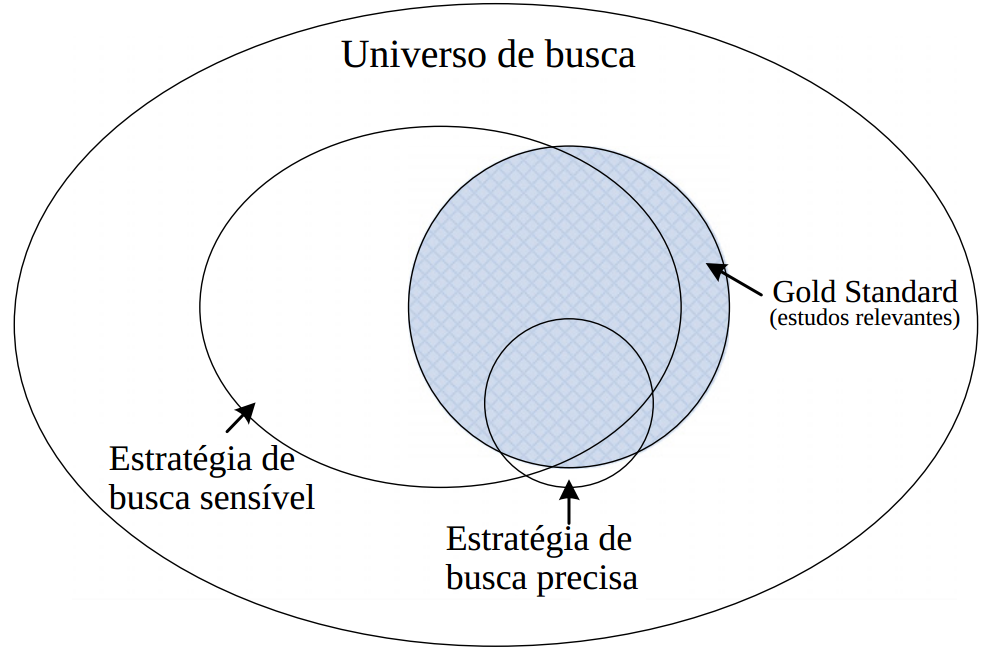
\includegraphics[scale=0.27]{figuras/gold_standard.png}    
    \caption{Busca sensível, precisa e \textit{gold standard}. Traduzido. Fonte: \citeauthor{zhang2011identifying}, \citeyear{zhang2011identifying}.}
    \label{fig:gold_standard}
\end{figure}


Uma estratégia de busca altamente precisa recuperará apenas uma pequena porção de estudos irrelevantes, mas pode perder um grande número de estudos do tipo \textit{gold standard}. Uma estratégia de busca perfeita seria 100\% sensitiva, bem como 100\% precisa, capturando exatamente o \textit{gold standard} sem quaisquer estudos irrelevantes \cite{zhang2011identifying}. A sensibilidade e precisão correspondente às strings de busca pode ser calculada como\cite{zhang2011identifying}:

$$Sensibilidade = \frac{\textit{\textrm{Número de estudos relevantes encontrados}}}{\textit{\textrm{Número total de estudos relevantes}}} \times 100\%$$

$$Sensitividade = \frac{\textit{\textrm{Número de estudos relevantes encontrados}}}{\textit{\textrm{Número de estudos encontrados}}} \times 100\% $$




\subsection{Ciclos de busca}

A construção das strings de busca podem ocorrer de dois modos: (i) definição subjetiva de string de busca e (ii) elicitação objetiva de termos de busca \cite{zhang2011identifying}. A primeira abordagem, a subjetiva, foi utilizada para definir a string do primeiro ciclo de busca. Tal string, foi definida baseada no conhecimento da pesquisadora e de seus orientadores. 

As strings dos demais ciclos de busca basearam-se na abordagem objetiva. O título, resumo e palavras-chave dos documentos em \textit{quasi-gold standard} são importados para o software de análise, neste caso, a ferramenta escolhida foi a \textit{Voyant Tools} (Seção \ref{susbsec:voyant}).
Esta ferramenta possibilitou obter strings recomendadas usando \textit{text mining}. Esta técnica é sugerida por  \citeonline{zhang2011identifying} e resulta em uma análise estatística das palavras ou frases que ocorrem com maior frequência nos estudos classificados como \textit{quasi-gold standard}; e que, consequentemente, melhor distinguirão estudos relevantes de irrelevantes.

\end{comment}

\subsection{Fluxo de atividades para Revisão Sistemática}

%sampaio2007

A Figura \ref{fig:processo_rs} ilustra o fluxo das atividades que orientou a execução da RS. Foi elaborado o protocolo de Revisão Sistemática definido no Apêndice \ref{appendix:protocolo}. O objetivo é disponibilizar os procedimentos e decisões do fluxo de atividades da RS realizado de modo que possa ser repetido por outros pesquisadores que obterão os mesmos resultados. A estrutura deste protocolo baseou-se no trabalho de \citeonline{ramaiane2014}.

\begin{figure}[!htb]
    \centering
    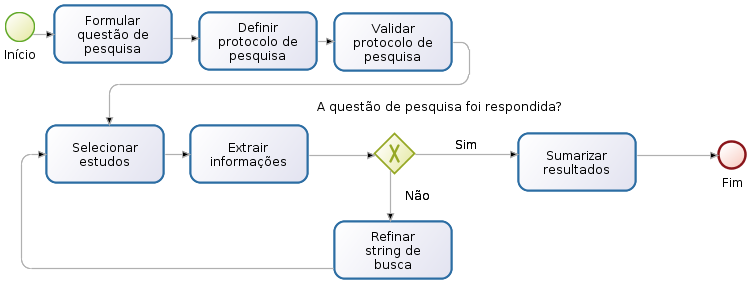
\includegraphics[scale=0.5]{figuras/processo_rs}
    \caption{Fluxo de atividades para Revisão Sistemática.}
    \label{fig:processo_rs}     
\end{figure}


\section{Metodologia de desenvolvimento} \label{sec:metodologia_desenvolvimento}

Foi adotada uma adaptação da metodologia Scrum para a atividade \textit{``Desenvolver padrões arquiteturais"} descrita na Figura \ref{fig:proc_tcc2}. 

\subsection{Scrum} \label{sec:scrum}

O Scrum é um \textit{framework}, no qual pode-se resolver problemas complexos de forma produtiva com o principal objetivo de gerar produtos de maior valor possível \cite{schwaber2016}. Isto é favorecido empregando-se uma abordagem iterativa e incremental que promove controle de riscos e uma melhor previsão dos mesmos. O Scrum fundamenta-se no empirismo, afirmando que o conhecimento é desenvolvido pela experiência. São três os pilares que sustentam a implementação do processo empírico:

\begin{enumerate}
    \item Transparência: aspectos significantes do fluxo devem ser visíveis para os responsáveis pelos resultados. A comunicação deve ser frequente e, consequentemente, estabelece confiança dos envolvidos;
    \item Inspeção: a transparência torna a inspeção possível. Envolve examinação atenciosa e \textit{feedbacks} constantes para tomar decisões com relação a adaptações no processo ou produto, e
    \item Adaptação: a inspeção torna a adaptação possível. Adaptação diz respeito aos ajustes no produto em desenvolvimento ou no processo; o qual está sendo desenvolvido de acordo com os resultados da inspeção \cite{rubin2012}.
\end{enumerate}

O objetivo do Scrum é entregar software de qualidade, tanto quanto possível, em intervalos curtos e fixos de tempo, intitulados \textit{Sprints} \cite{beedle1999}. Cada fase do ciclo de desenvolvimento de software - consideradas por \citeonline{beedle1999} como requisitos, análise, projeto, evolução e entrega - é mapeada para uma \textit{Sprint} ou conjunto de \textit{Sprints} \cite{beedle1999}. 

Além da \textit{Sprint}, existem outros eventos prescritos no Scrum: \textit{Sprint Planning, Daily Scrum, Sprint Review, Sprint Retrospective}. Estes eventos são usados para criar regularidade de encontros do time bem como minimizar a necessidade de reuniões não definidas no Scrum. Cada um desses eventos requer que seja estabelecida uma duração máxima \cite{beedle1999}.

Para definir se o que foi produzido é potencialmente entregável, o \textit{Scrum Team} deve ter a definição de pronto - \textit{Definition of Done} (DoD) - bem estabelecida. A definição de pronto é uma \textit{checklist} de tipos de trabalho que o time deve realizar completamente para declarar o trabalho desenvolvido na \textit{Sprint} como pronto \cite{rubin2012}.

Cada \textit{Sprint} opera com um certo número de itens de trabalho, constituindo o \textit{Backlog}. Os papéis responsáveis pelo processo representam o \textit{Scrum Team}. Este é constituído por: \textit{Product Owner}, \textit{Development Team}, e um \textit{Scrum Master} \cite{beedle1999}.

\subsection{Fluxo de atividades de desenvolvimento}\label{sec:proc_ds}

Foram realizadas adaptações no \textit{Scrum} devido ao fato de haver somente um membro na equipe para compor o \textit{Scrum Team}. Portanto, foram utilizados: entregas a cada \textit{Sprint}, cerimônia \textit{Sprint Planning} e a utilização do \textit{Definition of Done}.
Foram adotados os procedimentos descritos na Figura \ref{fig:proc_desenv}. As \textit{Sprints} tiveram duração de duas semanas, de modo que as estórias de usuário foram dadas como prontas seguindo a definição de pronto - ou \textit{Definition of Done} (ou ``DoD"). 

\newpage
\begin{figure}[!htb]
    \centering
    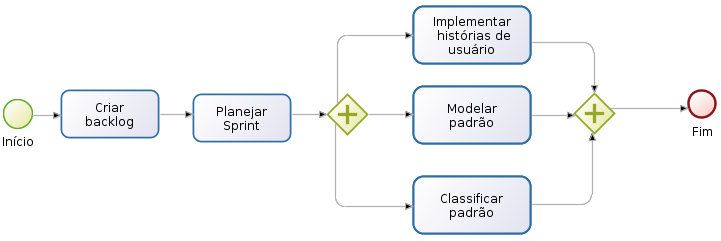
\includegraphics[scale=0.5]{figuras/processo_desenvolvimento.png}
    \caption{Fluxo de atividades para o desenvolvimento de software.} 
    \label{fig:proc_desenv}
\end{figure}



\input{principal/cronograma}

\section{Considerações parciais}

Esse capítulo teve como intuito apresentar os métodos utilizados no desenvolvimento desse trabalho. Ele contém as escolhas metodológicas, bem como os fluxos de atividades modelados que guiaram a condução deste. Elaborou-se um protocolo de condução da Revisão Sistemática, e foi apresentada uma visão temporal das atividades, por meio de cronogramas.